% This is text associated with the open textbook "Open Electromagnetics"
% See immediately below for author, date
% This work is licensed under the Creative Commons Attribution-ShareAlike 4.0 International License. (CC BY SA 4.0) 
% To view a copy of the license, visit http://creativecommons.org/licenses/by-sa/4.0/

%ORB TITLE Magnetic Field of an Infinitely-Long Straight Current-Bearing Wire
%ORB AUTHOR 0        # S.W. Ellingson, Virginia Tech (ellingson@vt.edu)
%ORB DATE 20180806   # yyyymmdd
%ORB ABSTRACT Magnetic Field of an Infinitely-Long Straight Line Current

\label{m0119_Magnetic_Field_of_a_Long_Wire} % <-- Must match name of this file and module directory name.  Don't mess with this!

In this section, we use the magnetostatic form of Ampere's Circuital Law 
\index{Ampere's law!magnetostatics}
(ACL) (Section~\ref{m0019_Amperes_Law_Magnetostatics}) to determine the magnetic field due to a steady current $I$ (units of A) in an infinitely-long straight wire.
The problem is illustrated in Figure~\ref{m0119_fLSW}.
The wire is an electrically-conducting circular cylinder of radius $a$.
Since the wire is a cylinder, the problem is easiest to work in cylindrical coordinates with the wire aligned along the $z$ axis.
%
\begin{figure}[b!]
\begin{center}
\pdftooltip{{  % note double braces
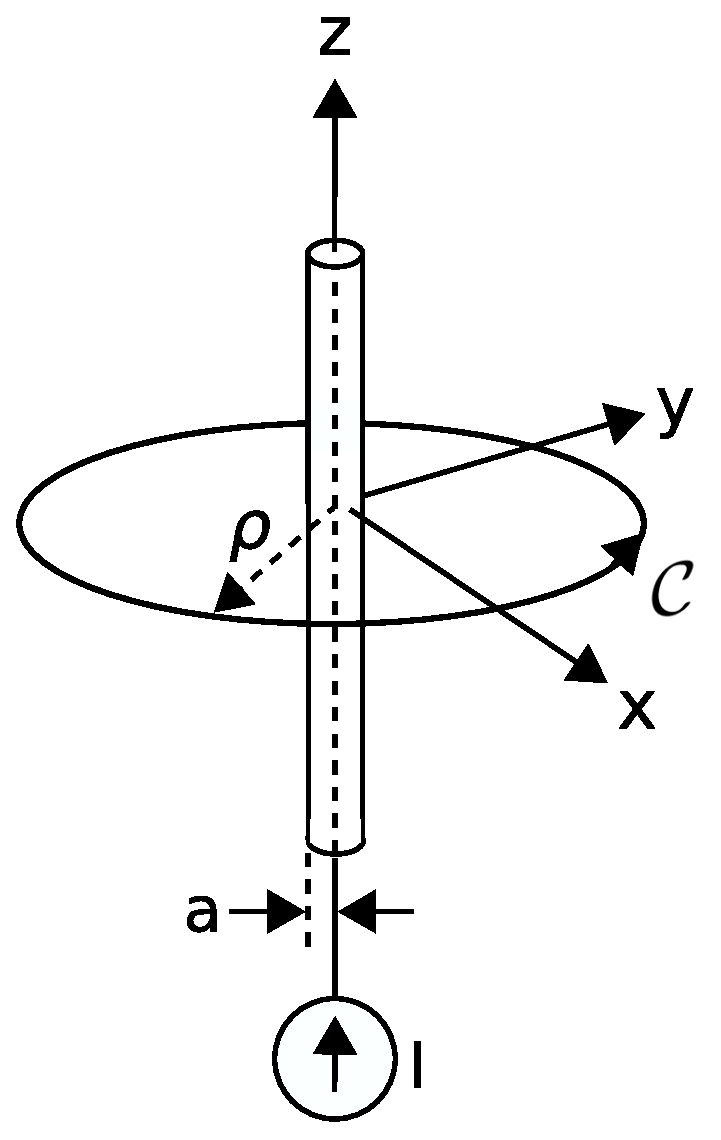
\includegraphics[width=2in]{modules/m0119_fLSW.eps}
% https://commons.wikimedia.org/wiki/File:M0119_fLSW.svg
}}{A small cylinder with radius a represents a wire, centered vertically on the z-axis in a Cartesian coordinate system. From the bottom, current is pointed upward through the wire. Around the middle of the wire is a circular path C, with an arrow on the path pointed counterclockwise to indicate direction. A dashed vector, rho, extends out of the middle of the wire to the left to the path, perpendicular to the z-axis.}
\end{center} 
\centerline{\scriptsize 
\copyright~\hyperref[m0119_fLSW_Credit]{K.\ Kikkeri} 
\href{https://creativecommons.org/licenses/by-sa/4.0/}{CC BY~SA 4.0} 
} 
\caption{
\label{m0119_fLSW}
Determination of the magnetic field due to steady current in an infinitely-long straight wire.
}
\end{figure}  

Here's the relevant form of ACL:
%
\begin{equation}   
\oint_{\mathcal C}{ {\bf H} \cdot d{\bf l} } = I_{encl}  
\label{m0119_eACL}
\end{equation}
%
where $I_{encl}$ is the current enclosed by the closed path ${\mathcal C}$.
ACL works for {\it any} closed path, so to exploit the symmetry of the cylindrical coordinate system we choose a circular path of radius $\rho$ in the $z=0$ plane, centered at the origin.  
With this choice we have 
%
\begin{equation}
I_{encl}=I ~~ \mbox{for}~\rho\ge a
\end{equation}

For $\rho<a$, we see that $I_{encl}<I$.  
a steady (DC) current will be distributed uniformly throughout the wire (Section~\ref{m0071_Resistance_DC}).
Since the current is uniformly distributed over the cross section, $I_{encl}$ is less than the total current $I$ by the same factor that the area enclosed by ${\mathcal C}$ is less than $\pi a^2$, the cross-sectional area of the wire.
The area enclosed by ${\mathcal C}$ is simply $\pi \rho^2$, so we have
%
\begin{equation}
I_{encl}
=I \frac{\pi \rho^2}{\pi a^2}
=I \frac{\rho^2}{a^2} ~~ \mbox{for}~\rho<a
\end{equation}
 
For the choice of ${\mathcal C}$ made above, Equation~\ref{m0119_eACL} becomes
%
\begin{equation}   
\int_{\phi=0}^{2\pi} { {\bf H} \cdot \left(\hat{\bf \phi}~\rho~d\phi\right) } = I_{encl}
\label{m0119_eACL1}
\end{equation}
%
Note that we have chosen to integrate in the $+\phi$ direction.
Therefore, the right-hand rule 
\index{right-hand rule!Stokes' theorem}
specifies that positive $I_{encl}$ corresponds to current flowing in the $+z$ direction, which is consistent with the direction indicated in Figure~\ref{m0119_fLSW}.
(Here's an excellent exercise to test your understanding. Change the direction of the path of integration and confirm that you get the same result obtained at the end of this section.  Changing the direction of integration should not change the magnetic field associated with the current!)

The simplest way to solve for ${\bf H}$ from Equation~\ref{m0119_eACL1} is to use a symmetry 
\index{symmetry}
argument, which proceeds as follows: 
%
\begin{itemize}
\item Since the distribution of current is uniform and infinite in the $z$-dimension, ${\bf H}$ can't depend on $z$, and so ${\bf H}\cdot\hat{\bf z}$ must be zero everywhere.
\item The problem is identical after any amount of rotation in $\phi$; therefore, the magnitude of ${\bf H}$ cannot depend on $\phi$. 
This is a form of radial symmetry.  
Since we determined above that ${\bf H}$ can't depend on $z$ either, it must be that the magnitude of ${\bf H}$ can depend only on $\rho$.  
\item The radial symmetry of the problem also requires that ${\bf H}\cdot\hat{\bf \rho}$ be equal to zero.  If this were not the case, then the field would not be radially symmetric.  Since we determined above that ${\bf H}\cdot\hat{\bf z}$ is also zero, ${\bf H}$ must be entirely $\pm\hat{\bf \phi}$-directed.
\end{itemize}
%
From the above considerations, the most general form of the magnetic field intensity can be written ${\bf H} = \hat{\bf \phi}H(\rho)$.  Substituting this into Equation~\ref{m0119_eACL1}, we obtain
%
\begin{flalign}   
I_{encl} &= \int_{\phi=0}^{2\pi} { \left[\hat{\bf \phi}H(\rho)\right] \cdot \left(\hat{\bf \phi}~\rho~d\phi\right) } \nonumber \\
         &= \rho H(\rho)~\int_{\phi=0}^{2\pi} { d\phi } \nonumber \\
         &= 2\pi \rho H(\rho)
\end{flalign}
%
Therefore, $H(\rho)=I_{encl}/2\pi \rho$.  Reassociating the known direction, we obtain:
%
\begin{equation}  
{\bf H}  = \hat{\bf \phi}\frac{I_{encl}}{2\pi \rho}
\end{equation}
%
Therefore, the field outside of the wire is:
%
\begin{equation} 
\boxed{  
{\bf H}  = \hat{\bf \phi}\frac{I}{2\pi \rho} ~~ \mbox{for} ~ \rho\ge a
}
\label{m0119_eACLLCe}
\end{equation}
%
whereas the field inside the wire is:
%
\begin{equation} 
\boxed{  
{\bf H}  = \hat{\bf \phi}\frac{I\rho}{2\pi a^2} ~~ \mbox{for} ~ \rho<a
}
\label{m0119_eACLLCi}
\end{equation}
%
(By the way, this is a good time for a units check.)

Note that as $\rho$ increases from zero to $a$ (i.e., inside the wire), the magnetic field is proportional to $\rho$ and therefore increases.
However, as $\rho$ continues to increase beyond $a$ (i.e., outside the wire), the magnetic field is proportional to $\rho^{-1}$ and therefore decreases.

If desired, the associated magnetic flux density can be obtained using ${\bf B} = \mu {\bf H}$.

Summarizing:
%
%ORB HIGHLIGHT
\begin{mdframed}[backgroundcolor=yellow!20,nobreak=true] 
The magnetic field due to current in an infinite straight wire is given by Equations~\ref{m0119_eACLLCe} (outside the wire) and \ref{m0119_eACLLCi} (inside the wire).
The magnetic field is $+\hat{\bf \phi}$-directed for current flowing in the $+z$ direction,
so the magnetic field lines form concentric circles perpendicular to and centered on the wire.
\end{mdframed}

Finally, we point out another ``right-hand rule'' 
\index{right-hand rule!magnetic field of a wire}
that emerges from this solution, shown in Figure~\ref{m0119_fRightHandRule} and summarized below:
%
%ORB HIGHLIGHT
\begin{mdframed}[backgroundcolor=yellow!20,nobreak=true] 
The magnetic field due to current in an infinite straight wire points in the direction of the curled fingers of the right hand when the thumb of the right hand is aligned in the direction of current flow. 
\end{mdframed}
%
This simple rule turns out to be handy in quickly determining the relationship between the directions of the magnetic field and current flow in many other problems, and so is well worth committing to memory.
%
\begin{figure}
\begin{center}
\pdftooltip{{  % note double braces
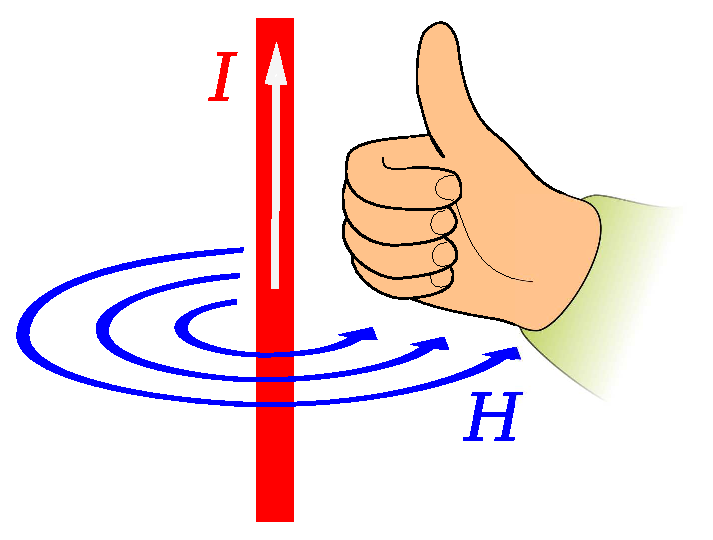
\includegraphics[width=2in]{modules/m0119_fRightHandRule.eps}
% https://et.wikipedia.org/wiki/Fail:Manoderecha.svg
}}{A red wire lies vertically, with a vector in the middle pointing up to represent current. Three blue, concentric circles lie around the middle of the rectangle, labeled H. To the right of the rectangle is a right hand, with the thumb pointed up and fingers curled. }
\end{center} 
\centerline{\scriptsize 
\copyright~\hyperref[m0119_fRightHandRule_Credit]{Jfmelero} 
\href{https://creativecommons.org/licenses/by-sa/4.0/}{CC BY~SA 4.0} (modified)
} 
\caption{
\label{m0119_fRightHandRule}
Right-hand rule for the relationship between the direction of current and the direction of the magnetic field.
}
\end{figure}  





